%%%%%%%%%%%%%%%%%%%%%%%%%
\section{الگوریتم‌های گراف}
%%%%%%%%%%%%%%%%%%%%%%%%%

\begin{frame}{‌الگوریتم‌های گراف}
\begin{itemize}\itemr
\item[-]
گراف یک ساختار گسسته است که با استفاده از آن می‌توان تعدادی مفهوم که با یکدیگر در ارتباط هستند را مدلسازی کرد.
\item[-]
برای مدلسازی مفاهیم از رئوس گراف و برای مدلسازی ارتباط بین مفاهیم از یال‌های گراف استفاده می‌کنیم.
\item[-]
گراف‌ها در علوم کامپیوتر و دیگر شاخه‌های علوم بسیار پر استفاده‌اند. برای مثال برای مدلسازی یک شبکهٔ کامپیوتری که از تعدادی کامپیوتر و تعدادی مسیر ارتباطی تشکیل شده است، می‌توانیم از یک گراف استفاده کنیم و از الگوریتم‌های گراف برای یافتن مسیر بهینه برای انتقال یک بسته در شبکه بهره بگیریم. همچنین در شبکه‌های اجتماعی می‌توان افراد و سازمان‌ها را به عنوان رئوس یک گراف در نظر گرفت و ارتباط بین افراد و سازمان‌ها را با استفاده از یال‌های گراف مدلسازی کرد. از الگوریتم‌های گراف جهت تحلیل این شبکه اجتماعی برای یافتن اطلاعات در گراف می‌توان استفاده کرد.
\end{itemize}
\end{frame}


\begin{frame}{‌الگوریتم‌های گراف}
\begin{itemize}\itemr
\item[-]
در زبان‌شناسی می‌توان از گراف‌ها جهت نمایش ارتباط بین کلمات در یک زبان استفاده کرد و از گراف به دست آمده در پردازش زبان طبیعی، و ترجمه‌های ماشینی استفاده کرد.
\item[-]
در علوم فیزیک و شیمی می‌توان از گراف‌ها جهت مدلسازی مولکول‌ها استفاده کرد و ساختار مولکول‌ها و روابط آنها و نیروهای بین اتم‌ها و مولکول‌ها را شبیه سازی کرد.
\item[-]
در علوم اجتماعی می‌توان از گراف‌ها جهت مدلسازی ارتباط انسان‌ها و نحوه منتشر شدن اطلاعات و افکار بین انسان‌ها و جوامع استفاده کرد.
\item[-]
در علوم زیست‌شناسی می‌توان از گراف‌ها جهت بررسی روابط بین گونه‌های جانوری و گیاهی و همچنین بررسی ساختار ژن‌ها استفاده کرد.
\end{itemize}
\end{frame}


\begin{frame}{‌الگوریتم‌های گراف}
\begin{itemize}\itemr
\item[-]
در این قسمت با روش‌های نمایش گراف و جستجوی گراف‌ها آشنا می‌شویم. با استفاده از روش‌های جستجوی گراف‌ها می‌توانیم ساختار یک گراف و ویژگی‌های آن را بشناسیم.
\end{itemize}
\end{frame}


\begin{frame}{‌الگوریتم‌های گراف}
\begin{itemize}\itemr
\item[-]
یک گراف را می‌توان با استفاده از دو مجموعهٔ رأس‌ها
\fn{1}{vertex set}
\m{(V)}
و یال‌ها
\fn{2}{edge set}
\m{(E)}
نمایش داد. بدین ترتیب دوتایی
\m{G = (V,E)}
گرافی را نمایش می‌دهد که در آن
\m{V}
مجموعه‌ای است از رئوس و
\m{E}
مجموعه‌ای است از یال‌ها. یک یال دو رأس را به یکدیگر متصل می‌کند.
\end{itemize}
\end{frame}


\begin{frame}{‌الگوریتم‌های گراف}
\begin{itemize}\itemr
\item[-]
علاوه بر روش استاندارد نمایش یک گراف توسط مجموعه‌ها، می‌توانیم یک گراف را توسط مجموعه‌ای از لیست‌های مجاورت
\fn{1}{adjacency lists}
یا یک ماتریس مجاورت
\fn{2}{adjacency matrix}
نشان دهیم.
\item[-]
توسط لیست مجاورت می‌توان گراف‌های خلوت
\fn{3}{sparse graph}
را که در آنها
\m{|E|}
بسیار کوچک‌تر از
\m{{|V|}^2}
است نمایش داد.
وقتی گراف متراکم
\fn{4}{dense}
است، می‌توان از نمایش ماتریس مجاورت استفاده کرد.
\end{itemize}
\end{frame}


\begin{frame}{‌الگوریتم‌های گراف}
\begin{itemize}\itemr
\item[-]
در نمایش لیست مجاورت
\fn{1}{adjacency-list representation}
برای گراف
\m{G = (V,E)}
از آرایهٔ
\m{Adj}
شامل
\m{|V|}
عنصر استفاده می‌کنیم. به ازای هر
\m{u \in V}
،
لیست مجاورت
\m{Adj[u]}
شامل رئوس
\m{v}
 است به طوری‌که
\m{(u,v) \in E}
. پس
\m{Adj[u]}
شامل همهٔ رئوسی است که در گراف
\m{G}
مجاور
\m{u}
هستند. در پیاده‌سازی این روش،
عناصر این آرایه می‌توانند اشاره‌گر به رئوس مجاور باشند.
\end{itemize}
\end{frame}


\begin{frame}{‌الگوریتم‌های گراف}
\begin{itemize}\itemr
\item[-]
در شکل زیر دو گراف توسط لیست مجاورت نشان داده شده‌اند.
\begin{figure}
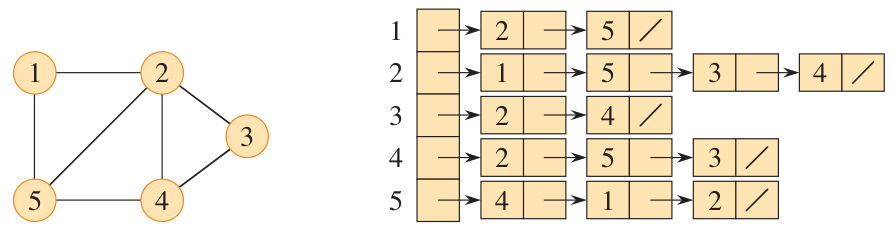
\includegraphics[width=0.6\textwidth]{figs/chap07/550-graph1-adj}
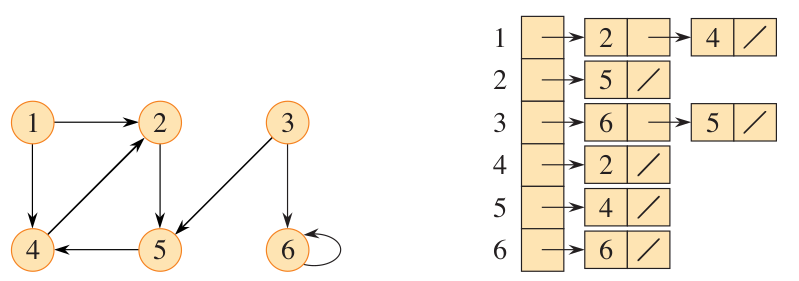
\includegraphics[width=0.6\textwidth]{figs/chap07/550-graph2-adj}
\end{figure}
\end{itemize}
\end{frame}


\begin{frame}{‌الگوریتم‌های گراف}
\begin{itemize}\itemr
\item[-]
اگر
\m{G}
یک گراف جهت‌دار باشد، مجموع اندازه همهٔ لیست‌های مجاورت برابراست با
\m{|E|}
، زیرا هریک از یال‌های
\m{(u,v)}
توسط درایهٔ
\m{Adj[u]}
نشان داده می‌شود.
\item[-]
اگر
\m{G}
یک گراف بدون جهت باشد، آنگاه مجموع اندازهٔ همهٔ لیست‌های مجاورت برابراست با
\m{2|E|}
، زیرا هر یک از یال‌های
\m{(u,v)}
هم در
\m{Adj[u]}
و هم در
\m{Adj[v]}
نمایش داده می‌شود.
\item[-]
فضای حافظه‌ای که لیست مجاورت برای نگهداری گراف نیاز دارد برابراست با
\ath{V+E} .
\iffalse
یافتن یک یال در گراف نیز به زمان
\ath{V+E}
نیاز دارد، زیرا برای یافتن یک یال همهٔ
\m{|V|}
درایهٔ لیست مجاورت باید بررسی شوند.
\fi
\end{itemize}
\end{frame}


\begin{frame}{‌الگوریتم‌های گراف}
\begin{itemize}\itemr
\item[-]
توسط لیست مجاورت می‌توانیم گراف‌های وزن‌دار
\fn{1}{weighted graphs}
را نیز نمایش دهیم.
در یک گراف وزن‌دار، هریک از یال‌ها دارای یک وزن است که توسط تابع وزن
\fn{2}{weight function}
\m{w : E \rightarrow \RR}
تولید می‌شود.
\item[-]
برای مثال فرض کنید
\m{G = (V,E)}
یک گراف وزن‌دار با تابع وزن
\m{w}
باشد. آنگاه می‌توانیم وزن
\m{w(u,v)}
از یال
\m{(u,v) \in E}
را در کنار رأس
\m{v}
در لیست مجاورت
\m{u}
ذخیره کنیم و نمایش دهیم.
\item[-]
یکی از معایب لیست مجاورت این است که برای پیدا کردن یال
\m{(u,v)}
سریع‌ترین روش ممکن جستجوی
\m{v}
در لیست مجاورت
\m{Adj[u]}
است.
\item[-]
ماتریس مجاورت برای پیدا کردن یک یال می‌تواند از لیست مجاورت سریع‌تر عمل کند.
\end{itemize}
\end{frame}


\begin{frame}{‌الگوریتم‌های گراف}
\begin{itemize}\itemr
\item[-]
در نمایش ماتریس مجاورت
\fn{1}{adjacency matrix representation}
برای گراف
\m{G = (V,E)}
فرض می‌کنیم هر رأس یک شماره از 
\m{1}
 تا
\m{|V|}
داشته باشد. سپس گراف
\m{G}
را با استفاده از ماتریس
\m{A = (a_{ij})}
با اندازهٔ
\m{|V| \times |V|}
نشان می‌دهیم به طوری‌که
\begin{align*}
\m{a_{ij}}  = \left\{ \begin{array}{lr}
				\m{1} & \m{(i,j) \in E}~\text{اگر}\\
					\m{0} & \text{در غیر اینصورت}
					\end{array}\right.
\end{align*}
\end{itemize}
\end{frame}


\begin{frame}{‌الگوریتم‌های گراف}
\begin{itemize}\itemr
\item[-]
در شکل زیر دو ماتریس مجاورت نشان داده شده‌اند.
\begin{figure}
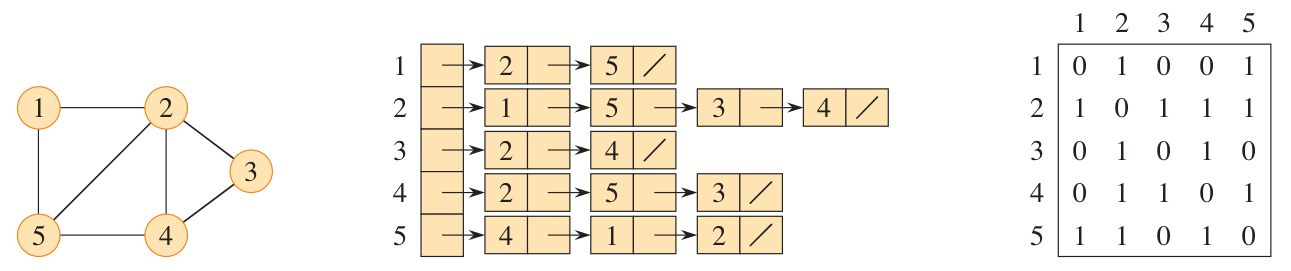
\includegraphics[width=0.9\textwidth]{figs/chap07/550-graph1}
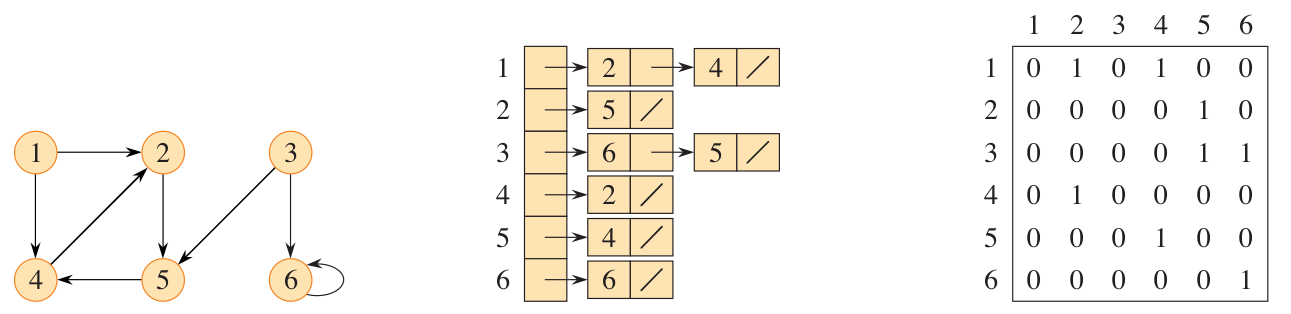
\includegraphics[width=0.9\textwidth]{figs/chap07/550-graph2}
\end{figure}
\end{itemize}
\end{frame}


\begin{frame}{‌الگوریتم‌های گراف}
\begin{itemize}\itemr
\item[-]
ماتریس مجاورت به حافظه
\ath{V^2}
برای نگهداری گراف نیاز دارد. برای یافتن یال
\m{(u,v)}
در گراف می‌توانیم درایهٔ
\m{A[u,v]}
را بررسی کنیم و بنابراین یافتن یک یال در گراف در زمان
\ath{1}
انجام می‌شود.
\item[-]
برای یک گراف بدون جهت، گراف نسبت به قطر اصلی‌اش متقارن است، زیرا
\m{A[u,v]}
برابراست با
\m{A[v,u]}
بنابراین ماتریس مجاورت برابر با ترانهادهٔ
\fn{1}{transpose}
 آن است و داریم
\m{A = A^T} .
\item[-]
اما در یک گراف جهت‌دار می‌توانیم یالی از
\m{u}
به
\m{v}
داشته باشیم بدون اینکه یال از
\m{v}
به
\m{u}
وجود داشته باشد.
\end{itemize}
\end{frame}


\begin{frame}{‌الگوریتم‌های گراف}
\begin{itemize}\itemr
\item[-]
با استفاده از ماتریس مجاورت می‌توانیم یک گراف وزن‌دار را نیز نمایش دهیم.
\item[-]
برای مثال، اگر
\m{G = (V,E)}
یک گراف وزن‌دار با تابع وزن
\m{w}
باشد، می‌توان وزن
\m{w(u,v)}
برای یال
\m{(u,v) \in E}
را به عنوان درایهٔ ماتریس مجاورت در سطر
\m{u}
و ستون
\m{v}
ذخیره کرد.
\item[-]
استفاده از ماتریس مجاورت در عمل راحت‌تر است اما به ازای گراف‌های بزرگ خلوت ممکن است فضای حافظه مورد نیاز آنها بسیار زیاد شود.
برای ذخیره‌سازی گراف‌های خلوت جهت‌دار، لیست مجاورت نسبت به ماتریس مجاورت فضای بسیار کمتری اشغال می‌کند.
\end{itemize}
\end{frame}